%!TeX root: thesis.tex
\section{Einleitung}
\subsection{Motivation} \label{motiv}
Als ich im Wintersemester das Modul "Compilerbau"\ 
belegt habe, habe ich mich das erste Mal mit
einigen Algorithmen beschäftigt, die eben in diesem
Themengebiet angewendet werden. Dabei fiel es mir
bei einigen schwer, mir diese ohne weiteres
vorzustellen. Ein Tool, mit dem man Schritt für Schritt 
durch diese Algorithmen gehen kann, hätte mir das Verstehen der Algorithmen
und vor allem das Entwickeln einer Intuition, warum diese Algorithmen überhaupt
so funktionieren wie sie es tun stark erleichtert.\\

Es gibt zwar solche Tools, zum Beispiel VisOpt\cite{VisOpt} oder DFAV\cite{dfav},
diese benutzen allerdings ein Subset von Java und JavaScript.
Da im Modul \glqq Compilerbau\grqq sämtliche Algorithmen auf drei Address Code
erklärt werden, passen diese Tools nicht in den Usecase der Studenten.\\

In dieser Bachelorarbeit wird ein Framework in Java
entwickelt, mit dem es einfach sein soll,
Algorithmen zu visualisieren.\\

Im Jahr 2016 wurde von Fabian Ruhland und Isabel Wingen bereits ein ähnliches
Framework entwickelt \cite{toolbox}. Dieses ist leider mittlerweile nicht mehr
mit aktuellen Java-Versionen kompatibel, daher wurde sich dazu entschieden,
ein komplett neues Framework zu entwickeln.\\

Zudem werden einige der Algorithmen, die im Compilerbau verwendet werden,
implementiert. Das Framework basiert darauf, dass durch
Implementierung von Interfaces einfach neue Algorithmen 
als Plugins hinzugefügt werden können. Dadurch kann gewährleistet werden,
dass wenn etwas im Framework nicht mehr funktioniert, 
zum Beispiel durch neue Versionen von Java oder einem Update einer Dependency, 
dieses Modul ausgetauscht werden kann, ohne die implementierten Plugins 
aktualisieren zu müssen.


\newpage
\subsection{Theoretische Grundlagen}
Im folgenden Abschnitt werden die für diese Arbeit notwendigen 
grundlegenden Konzepte und Algorithmen erklärt, da im weiteren 
Verlauf der Arbeit nur auf die Implementierung dieser eingegangen wird.


\subsubsection{Drei Adress Code} \label{t:tac}
Drei Adress Code ist eine Art von Zwischencode
\footnote{Zwischencode hat viele Nutzungsgebiete in einem Compiler,
einerseits verbindet er das Frontend (welches den Quellcode einließt) mit dem
Backend (welches den Maschinencode ausgibt), andererseits ist Zwischencode 
plattformunabhängig, sodass maschinenunabhängige Optimierungen und Analysen auf
diesem ausgeführt werden können.}. 
Charakterisierend für Drei Adress Code (folgend auch 3-Address-Code genannt)
ist, dass einzelne Instruktionen auf maximal drei Adressen (oder Konstanten) 
zugreifen. Die Addresse in die der resultierende Wert gespeichert wird und 
eine oder zwei Addressen oder Konstanten aus denen sich der resultierende Wert bildet.
Dazu ist noch die Operation, die ausgeführt wird angegeben.\\

Für diese Bachelorarbeit wurde eine Teilmenge des im Drachenbuch \cite[Kapitel 6.2.1]{D}
beschriebenen 3-Address-Code verwendet.\\
Folgende Operationen gibt es:
\begin{enumerate}
  \item Binäre Operationen X = Y op Z\\
    in denen das Resultat aus einer der folgenden binären Operation
    in der Adresse X gespeichert wird. Implementiert wurden Addition, 
    Subtraktion, Multiplikation und Division.
  \item Die unäre Operation X = - Y\\
    in der der invertierte Wert von Y in X gespeichert wird.
  \item Der Kopierbefehl X = Y\\
    in der der Wert, der in Adresse Y gespeichert ist, in X kopiert wird.
  \item Der unbedingte Sprung goto X\\
    hier wird kein Wert gespeichert, sondern zu der Adresse die in X gespeichert ist gesprungen
  \item Die bedingten Sprünge if Y goto X und ifFalse Y goto X\\
    mit denen, wenn der Wert Y entweder $wahr$ oder $falsch$ repräsentiert 
    zur Adresse X gesprungen wird  
    oder die nächste Instruktion ausgeführt wird, wenn dies nicht der Fall ist.
  \item Die bedingten Sprünge if Y relOp Z goto X\\
    in denen auch zu X gesprungen wird, wenn die Relation Y relOp Z $wahr$ ist, 
    sonst wird auch hier die nächste Instruktion ausgeführt.\\
    Die Implementierten Relationen sind: 
    \begin{itemize}
      \item Y $<$ Z
      \item Y $\leq$ Z
      \item Y $>$ Z
      \item Y $\geq$ 
      \item Y $=$ Z
      \item Y $\neq$ Z
    \end{itemize}
\end{enumerate}

Hierbei können die Adressen X, Y und Z beliebige Zeichenfolgen sein, 
Y und Z können außerdem Konstanten sein.
Die einzelnen Elemente jeder Instruktion sind durch ein Leerzeichen von einander
getrennt. Verschiedene Instruktionen werden durch einen Zeilenumbruch getrennt.
Da sich die Algorithmen in dieser Arbeit nicht mit komplexeren Aufgaben wie
Speichermanagement beschäftigen, wurde sich dagegen entschieden, den 3AC
umfangreicher zu modellieren.\\

Ein Beispiel für gültigen 3-Address-Code wäre also:
\begin{lstlisting}[caption={3-Address-Code, der die 5-te Fibonacci Zahl ausrechnet und in x speichert}]
  0: n = 5
  1: fib = 1  
  2: lst = 1
  3: n = n - 2
  4: if n <= 0 goto 10
  5: hlp = lst 
  6: lst = fib
  7: fib = lst + hlp
  8: n = n - 1
  9: goto 4
 10: x = fib
\end{lstlisting}


\subsubsection{Grundblöcke} \label{t:bb}
Grundblöcke sind Instruktionsfolgen eines Zwischencodeprogramms,
die immer zusammen ausgeführt werden \cite[S.619]{D}.
Dies ermöglicht es, einen Block an Instruktionen anzuschauen 
und bestimmte Optimierungsalgorithmen auf sie anzuwenden, 
ohne Gefahr zu laufen, die Semantik des Programmes zu verändern.

\newpage
Um ein Programm in Grundblöcke aufzuteilen, kann man wie folgt vorgehen \cite[S.643]{D}:
\begin{enumerate}
  \item Markiere die erste Instruktion des Programmes als Leader, da diese immer ausgeführt wird.
  \item Markiere alle Instruktionen als Leader, die Ziel eines Sprungs sind oder auf einen Sprung folgen.
  \item Alle Instruktionen, die auf eine markierte Instruktion folgen
    bis zu einer neuen markierten Instruktion, gelten nun als ein Grundblock.
\end{enumerate}

Folgend kann man für jeden Grundblock bestimmen, welche Grundblöcke auf ihn folgen, 
daraus lässt sich ein Flussgraph bestimmen, den wir, da er den Kontrollfluss beschreibt,
folglich Kontrollflussgraphen nennen werden. In diesem stellt jeder Grundblock einen Knoten dar
und jede Kante einen Sprung von einem Grundblock zum anderen.\\

Aus unserem Beispielcode aus dem letzten Kapitel können wir also folgende Instruktionen markieren:
\begin{lstlisting}[caption=Fibonacci 3-Address-Code mit markierten Leadern]
  0: n = 5 //Leader, da erste Instruktion
  1: fib = 1  
  2: lst = 1
  3: n = n - 2
  4: if n <= 0 goto 10 //Leader, da 9 hierhin springt
  5: hlp = lst //Leader, da 4 ein bedingter Sprung ist
  6: lst = fib
  7: fib = lst + hlp
  8: n = n - 1
  9: goto 4
 10: x = fib //Leader, da 9 ein Sprung ist und 4 hierhin springen kann
\end{lstlisting}

Daraus folgt, dass wir folgende Grundblöcke haben:
\begin{enumerate}
  \item Ein Grundblock $B_0$, der die Addressen 0 bis 3 besitzt,
  \item der Block $B_1$, der nur die Addresse 4 hat,
  \item Grundblock $B_2$, der die Addressen 5 bis 9 besitzt
  \item und Block $B_3$, der nur die Addresse 10 besitzt.
\end{enumerate}




\newpage
\subsubsection{Kontrollflussgraphen}
Kontrollflussgraphen sind gerichtete Graphen, deren Knoten aus Grundblöcken und 
deren Kanten aus den jeweilig folgenden Grundblöcken besteht.\\

Um unser Beispiel weiterzuführen, bildet sich folgender Kontrollflussgraph:
\begin{figure}[h]
  \centering
  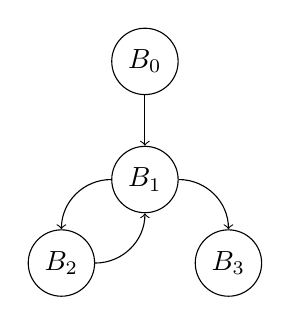
\begin{tikzpicture}[node distance={15mm}, 0/.style = {draw, circle}]
    \node[0] (0) {$B_0$};
    \node[0] (1) [below of=0] {$B_1$};
    \node[0] (2) [below left of=1] {$B_2$};
    \node[0] (3) [below right of=1] {$B_3$};
    \draw[->] (0) to [out=270, in=90] (1);
    \draw[->] (1) to [out=180, in=90] (2);
    \draw[->] (1) to [out=0, in=90] (3);
    \draw[->] (2) to [out=0, in=270] (1);
  \end{tikzpicture}
  \caption{Resultierender Kontrollflussgraph}
  \label{fig:fib-cfg}
\end{figure}

Auf Kontrollflussgraphen lassen sich nun sogenannte Datenflusswerte definieren.
Diese sind Abstraktionen für die Menge aller möglichen Zustände des Programmes
zu einem bestimmten Zeitpunkt. In Bezug zu einem Kontrollflussgraphen ist dieser
Zeitpunkt immer entweder (direkt) vor der Ausführung des Grundblockes, die $in[B]$ Menge
oder nach der Ausführung dessen, die $out[b]$ Menge.
Je nach dem, was wir analysieren beziehungsweise abstrahieren wollen, ändern sich
die Datenflusswerte, da nur die für die jeweilige Analyse relevanten Informationen
betrachtet werden. Ausserdem abhängig von der spezifischen Analyse ist die
Flussrichtung der Datenflusswerte. Wenn der Datenfluss vorwärts gerichtet ist,
verändert sich die $out[B]$ Menge durch Anwendung einer sogenannten Transferfunktion
auf der $in[B]$ Menge, also gilt:
\[out[B]=f_B(in[B])\] 
\[in[B]=\bigcup_{v\in V_B}out[v]\]
Analog gilt, wenn der Datenfluss
rückwärtsgerichtet ist: 
\[in[B]=f_b(out[B])\]
\[out[B]=\bigcup_{n\in N_B}in[n]\]
Hierbei sind $V_B$ und $N_B$ die Mengen der Vorgänger und Nachfolger
eines Grundblocks $B$.\cite[S.732-734]{D}



\newpage
\subsubsection{Erreichende Definitionen} \label{t:rd}
Dies ist eine der gebräuchlichsten und nützlichsten Datenflussanalysen \cite[S.734]{D}.\\
Mit ihnen können wir herausfinden, welchen Variablen zu einem bestimmten
Zeitpunkt ein Wert zugewiesen ist. Eine Anwendung wäre zum Beispiel zu
kontrollieren, ob eine Variable zu einem bestimmten Zeitpunkt  überhaupt
einen Wert hat \cite[S.734]{D}, sofern die ursprüngliche Programmiersprache dies als 
notwendig erachtet. Man kann aber auch schauen, 
ob die Variable eine Konstante ist und somit Instruktionen gespart werden können.

Für die Berechnung der erreichenden Definitionen bestimmen 
wir folgende Datenflusswerte für jeden Grundblock:
\begin{itemize}
  \item Die $gen_B$ Menge\\
    beschreibt die Adressen aller Instruktionen in einem Grundblock $B$ welche einer Variable einen Wert zuweisen,
    also einen Wert \textit{generieren}. Wenn einer Variable ein Wert mehrmals zugewiesen wurde 
    liegt nur die letzte Zuweisung dieser in der $gen_B$ Menge.
  \item Und die $kill_B$ Menge\\
    beschreibt die Adressen aller Instruktionen welche einer Addresse einen Wert zuweisen, 
    der durch eine Instruktion in der $gen_B$ Menge überschrieben wird.
\end{itemize}

Nun können wir uns herleiten, dass alle Variablen, die in einem Grundblock $B$
definiert werden, ihn auch verlassen, also Teil der $out[B]$ Menge sind.
Zudem verlassen auch alle Definitionen den Grundblock, wenn sie nicht überschrieben wurden.
Demnach ist der Datenfluss vorwärtsgerichtet und es gilt die Transferfunktion:
\[out[B]=gen_B \cup (in[B] \backslash kill_B)\]
Hierbei handelt es sich um einen Fixpunktalgorithmus. Das heißt, wir beginnen
mit $out[B]=\emptyset$ für alle Grundblöcke und iterieren dann so lange über diese,
bis sich keine Menge mehr verändert.\cite[S.739-740]{D}

Für unser Beispiel ergibt sich dann \cref{tab:fib-rd}:

\newpage
\begin{table}[h]
  \centering
  \begin{tabular}{|l|c|c|c|c|}
    \hline
    $B       $&$B_0      $&$B_1          $&$B_2          $&$B_3            $\\\hline
    $gen_B   $&$1,2,3    $&$             $&$5,6,7,8      $&$10             $\\\hline
    $kill_B  $&$0,6,7,8  $&$             $&$1,2          $&$               $\\\hline
    $ in_1[B]$&$         $&$             $&$             $&$               $\\\hline
    $out_1[B]$&$\textcolor{hhudarkblue}{n,fib,lst}$&$$&$\textcolor{hhudarkblue}{n,fib,lst,hlp}$&$\textcolor{hhudarkblue}{x}$\\\hline
    $ in_2[B]$&$         $&$\textcolor{hhudarkblue}{n,fib,lst,hlp}$&$$&$          $\\\hline
    $out_2[B]$&$n,fib,lst$&$\textcolor{hhudarkblue}{n,fib,lst,hlp}$&$n,fib,lst,hlp$&$x$\\\hline
    $ in_3[B]$&$         $&$n,fib,lst,hlp$&$\textcolor{hhudarkblue}{n,fib,lst,hlp}$&$\textcolor{hhudarkblue}{n,fib,lst,hlp}$\\\hline
    $out_3[B]$&$n,fib,lst$&$n,fib,lst,hlp$&$n,fib,lst,hlp$&$x,\textcolor{hhudarkblue}{n,fib,lst,hlp}$\\\hline
    $ in_4[B]$&$         $&$n,fib,lst,hlp$&$n,fib,lst,hlp$&$n,fib,lst,hlp  $\\\hline
    $out_4[B]$&$n,fib,lst$&$n,fib,lst,hlp$&$n,fib,lst,hlp$&$x,n,fib,lst,hlp$\\\hline
  \end{tabular}
  \caption{Erreichende Definitionen für Fibonacci. Veränderungen sind \textcolor{hhudarkblue}{blau} markiert}
  \label{tab:fib-rd}
\end{table}

\subsubsection{Lebendige Variablen} \label{t:la}
Bei der Analyse lebendiger Variablen (folgend auch liveness Analyse genannt)
bringen wir in Erfahrung, ob ein bestimmter Wert zu einem bestimmten Zeitpunkt lebendig ist.
Lebendig bedeutet in diesem Kontext, dass dieser Wert definiert wurde
und zu einem späteren Zeitpunkt im Programm auch noch genutzt wird.\\

Die Analyse lebendiger Variablen hat viele Anwendungsgebiete. 
Beispielsweise bei der Registervergabe:\\
Ein reeller Computer hat nur eine begrenzte Anzahl an Registern.
Somit können nicht unendlich viele Variablen gleichzeitig in einem Register zur Verfügung stehen.\\
Im worst case Szenario bedeutet das, dass alle Werte nach ihrer Berechnung
in den Speicher geschrieben werden müssen und vor jeder Berechnung aus dem
Speicher geladen werden müssen.\\
Da dies viel mehr Zeit kostet als Werte, welche wieder genutzt werden,
bis dahin in einem Register zu lassen
\footnote{Wir sparen also das Speichern in einer Adresse und das Laden aus einer Adresse},
ist es sinnvoll, Interaktionen mit dem Speicher so gering wie möglich zu halten.\\
Die liveness Analyse kann hier berechnen wie viele Register wir maximal benötigen,
da eventuell nicht alle Variablen gleichzeitig lebendig sind, also gleichzeitig benötigt werden.\\
(Frei nach dem Drachenbuch\cite[S.743-744]{D} zitiert.)

\newpage
Auch für die liveness Analyse auf Grundblöcken
\footnote{Die liveness Analyse kann auch auf einzelnen Instruktionen ausgeführt werden.
In Kapitel 3.5 wird dies erneut aufgegriffen und erläutert.}
definieren wir wieder zwei Mengen, welche wir
für die Transferfunktion benötigen \cite[S.743]{D}:

\begin{enumerate}
  \item Die $def_B$ Menge\\
    in der $def_B$ Menge sind alle Variablen enthalten, denen im Gundblock $B$ ein Wert zugewiesen wird,
    bevor diese "verwendet" wird. Das bedeutet dass wir alle Variablen in dieser Menge zu Beginn des Blockes
    als "tot" betrachten können.
  \item Die $use_B$ Menge\\
    die $use_B$ Menge definiert alle Variablen, deren Werte vor ihrer Definition verwendet werden.
    Dementsprechen sind alle Variablen in dieser Menge zu beginn des Grundblockes "lebendig".
\end{enumerate}

Daraus bilden wir uns eine rückwärtsgerichtete Transferfunktion:
\[in[B]=use_B\cup (out[B]\backslash def_B)\]
Da nur die Variablen zu Beginn der Ausführung von Grundblock $B$,
leben müssen welche benutzt werden oder in einem Nachfolger benutzt werden, 
aber nicht in diesem Block definiert werden.\\

In unserem Beispiel resultiert dies in folgenden Mengen:
\begin{table}[h]
  \centering
  \begin{tabular}{|l|c|c|c|c|}
    \hline
    $B       $&$B_0      $&$B_1          $&$B_2      $&$B_3           $\\\hline
    $def_B   $&$n,fib,lst$&$             $&$hlp      $&$x             $\\\hline
    $use_B   $&$         $&$n            $&$lst,fib,n$&$fib           $\\\hline
    $out_1[B]$&$         $&$             $&$         $&$              $\\\hline
    $ in_1[B]$&$         $&$\textcolor{hhudarkblue}{n}$&$\textcolor{hhudarkblue}{lst,fib,n}$&$\textcolor{hhudarkblue}{fib}$\\\hline
    $out_2[B]$&$\textcolor{hhudarkblue}{n}$&$\textcolor{hhudarkblue}{lst,fib,n}$&$\textcolor{hhudarkblue}{n}$&$$\\\hline
    $ in_2[B]$&$         $&$n,\textcolor{hhudarkblue}{lst,fib}$&$lst,fib,n$&$fib$\\\hline
    $out_3[B]$&$n,\textcolor{hhudarkblue}{lst,fib}$&$lst,fib,n$&$lst,fib,n$&$$\\\hline
    $ in_3[B]$&$         $&$n,lst,fib$&$lst,fib,n$&$fib$\\\hline
    $out_4[B]$&$n,lst,fib$&$lst,fib,n$&$lst,fib,n$&$$\\\hline
    $ in_4[B]$&$         $&$n,lst,fib$&$lst,fib,n$&$fib$\\\hline
  \end{tabular}
  \caption{Liveness Analyse für unser Fibonacci Programm. Veränderungen sind \textcolor{hhudarkblue}{blau} markiert}
  \label{tab:fib-lab}
\end{table}


Dies sind alle theoretischen Grundlagen, die für das Verstehen der in dieser
Arbeit implementierten Konzepte benötigen, wenden wir uns nun der Implementierung zu.
